\documentclass[a4paper, 12pt]{article}
\usepackage{graphicx}
\usepackage{caption}
\usepackage{wrapfig}
\usepackage{float}
\usepackage{cmap}
\usepackage{tikz}
\usepackage{enumitem}
\usepackage{multirow}
\usepackage[utf8]{inputenc}
\usepackage[english, russian]{babel}
\usepackage{amsmath, amsfonts, amssymb, amsthm, mathtools}

\title{ЗАКОН ПАШЕНА}
\date{}

%-----------------------------------СOLONTITLE-------------------------------------------

\usepackage{fancyhdr}

   \pagestyle{fancy}
   \fancyhead{}
   \fancyhead[L]{ВПВ}
   \fancyhead[R]{Грошев Максим}
   \fancyfoot[C]{\thepage}

%------------------------------------------------------------------------------------------
\usepackage{extsizes}
\begin{document}

%-----------------------------------TITLEPAGE-----------------------------------------------

    \begin{titlepage}
    \maketitle
    \thispagestyle{empty}

            \begin{figure*}[h]
            \centering
            
\includegraphics[scale=1.3]{./pics/rt.png}
            \end{figure*}

             \vspace{15em}
             \begin{flushright}
                 \normalsize Выполнил:\\
                             Грошев М.А. Б01-206
             \end{flushright}

             \begin{center}
                    \vfill \normalsize Долгопрудный 2023
             \end{center}
    \end{titlepage}

%-------------------------------------------------------------------------------------------

\newpage
\setcounter{page}{1}

\textbf{Цель работы:}  Исследовать закон Пашена и определить границы его применимости.\\

%--------------------------------------------THEORY------------------------------------------

\section{Исторические сведения}


\begin{wrapfigure}{left}{0.5\textwidth}
	\vspace{-10pt}
	\centering
	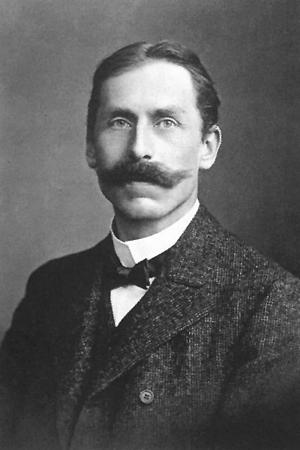
\includegraphics[width=0.4\textwidth]{ pics/pashen.jpg}
	\caption{Фридрих Пашен (1865-1947).}
	\label{img:plasma probe}
\end{wrapfigure}

Немецкий физик, иностранный почетный член АН СССР (1930). Отметился трудами электрическим разрядам в
газах (установил закон, названный его именем, 1889), спектроскопии, спектральным и
измерительным приборам. Обнаружил спектральную серию водорода в инфракрасной области.
\\ \\ \\ \\ \\ \\ \\ \\ \\ \\


%-------------------------------------------------------------------------------------------

\section{Закон Пашена}

\textit{Разность потенциалов $\varphi$ между электродами трубки, при которой начинается пробой газа, есть
функция произведения давления газа $P$ на расстояние между электродами $l$.}
\par
\textbf{Электрический пробой} - явление резкого возрастания тока в твёрдом, жидком или
газообразном диэлектрике (или полупроводнике) или воздухе, возникающее при приложении напряжения
выше критического.

\newpage
\subsection{Доказательство закона Пашена}

%-------------------------------------------------------------------------------------------

\subsubsection{Опыт Таунсенда}

Введём два коэффициента ионизации $\alpha$, $\beta$
\newline \par
$\alpha$ - среднее число ионов одного знака, производимое электроном на еденице пути длины
своего пути. Аналогичный смысл имеет имеет коэффициент $\beta $, характеризующий ионизирующую
способность положительных ионов. Причём  $\alpha > \beta$\newline
\begin{wrapfigure}{left}{0.5\textwidth}
	\vspace{-10pt}
	\centering
	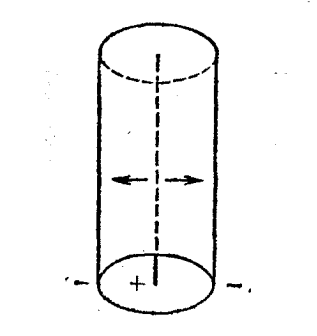
\includegraphics[width=0.4\textwidth]{ pics/setup.png}
	\caption{Установка опыта Таунсенда}
\end{wrapfigure}

Что доказывается следующим экспериментом. Берется нонизационная камера
в внде цилидрического
конденсатора, внутренним электродом которого служит тонкая
металлическая нить. Между нитью и наружным цилиндром конденсатора
прикладывается разность потенциалов $U$, достаточная для того, чтобы в объеме
камеры происходила ударная ионизация газа. Последняя практически
будет происходить лишь вблизи
нити, где электрическое поле очень сильное. Допустим, что на нить
подан положительный потенциал. Тогда к нити устремятся элек-
троны и будут вблизи нее ионизовать газ. Положительные же ионы,
устремляясь к наружному цилиндру, пройдут через область слабого
поля и практически никакой ионизации не вызовут. Изменим теперь
полярность напряжения $U$, не меняя его величину. Тогда роли
положительных и отрицательных ионов поменяются местами. К нити
устремятся положительные ионы, и ионизация в камере будет воз
буждаться практически только ими. Опыт показывает, что в первом случае ионизационный ток больше и быстрее растет с напряжением $U$, чем во втором.
\begin{figure}[H]
        \centering
        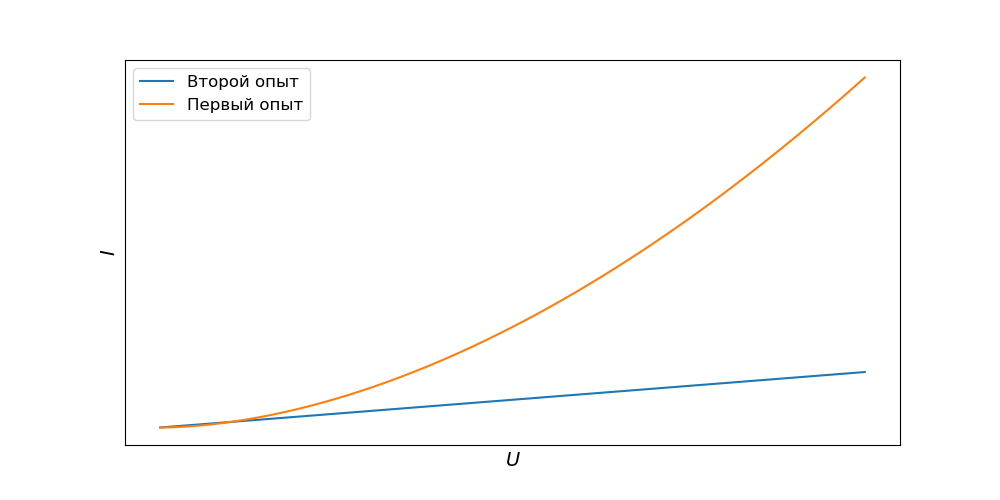
\includegraphics[scale=0.55]{./pics/taus.png}
        \caption{Результат опыта Таунсенда}
\end{figure}

%-------------------------------------------------------------------------------------------

\subsubsection{Зависимость $\alpha$, $\beta$ от $E$, $P$}

Для определенности рассмотрим электроны. Примем вместе, что при каждом столкновении
электрон теряет скорость, которую он приобрел в электрическом поле.
Чтобы электрон мог ионизовать газ, он должен на пути свободного пробега х приобрести
энергию, не меньшую энергии ионизации, т. е. величина $x$
должна удовлетворять условию:\\
\begin{equation*}
    xE \geq U_{ion},
\end{equation*}
\\
где $U_{ion}$; — потенциал ионизации. Предположим, что каждый такой электрон будет ионизировать газ.
Пустим тогда почок из $N_0$ электронов в поле $E$ c нулевой начальной скоростью. Известно, что
среднее число электронов, проходящих путь $x$ без столкновений:
\begin{equation*}\\
    N = N_0\cdot e^{\frac{-x}{\overline l}}
\end{equation*}
\\
где $\overline l$ - средняя длина свободного пробега электрона. Рассмотрим крайний случай:
$ xE = U_{ion}$. В таком случае на пути 1 см электрон испытает $\frac{1}{\overline l}$
столкновений. Тогда получим, что на всём пути у нас будет следующее число ионизаций\\
\begin{equation}
    \frac{N}{\overline l} = \frac{N_0}{\overline l}\cdot e^{\frac{-x}{\overline l}}
\end{equation}
\\
Тогда из получеенного выражения уже будет несложно получить выражение для среднего числа
ионизаций, проводимых одним электроном на том же пути\\
\begin{equation}
    \alpha = \frac{1}{\overline l}\cdot e^{\frac{U_{ion}}{E \overline l}}
\end{equation}
\\
Полуьзуясь тем фактом, $\overline l = \frac{1}{AP}$, где A - некоторая константа
\\
\begin{equation}
    \alpha = AP \cdot e^{{BP}{E}},
\end{equation}
\\
где В - некоторая константа. Отсюда получаем:\\
\begin{equation}
    \frac{\alpha}{P} = f(\frac{E}{P}),
\end{equation}
\\
Данное выражение позже было проверено Таунсендом для ряда газов при малых далениях ($P < P_{atm}$). Однако позже
Показано, что данное соотношение дает ошибку при давлениях больших атмосферного, а при больших
давлениях ($P >> P_{atm}$) становится неверным.
\par
Если продифференцировать данное выражение и найти его максимум, то получим, что он достигается
при $P = \frac{E}{B}$ и равен:\\
\begin{equation}
    \alpha_{max} = \frac{A}{eB}E,
\end{equation}
\\
где e - основание натурального логорифма. Т.о максимальное значение ионизируемости пропорционально
напряжению электрического поля.


%-------------------------------------------------------------------------------------------

\subsubsection{Условие пробоя}
Из теории построенной Таунсендом, монжно получить условие пробоя газа или зажигания
газового разряда.\\
\begin{equation}
    (\beta + \gamma \cdot \alpha)e^{(\beta + \alpha)l} - (1 + \gamma)\alpha = 0
\end{equation}
\\
Рассмотрим случай, когда вторичная эмиссия электронов у катода роли не играет $(\gamma = 0)$
Тогда подстявлаяя в 6, следующие выражения:\\
\begin{equation*}
    \alpha = P f (\frac{U}{lP})
\end{equation*}
\begin{equation*}
    \beta = P f_1 (\frac{U}{lP}),
\end{equation*}
\\
где $U$ напряжение на трубке. Тогда несложно получить следующее выражение.\\
\begin{equation*}
    F(\frac{U}{lP}) = 0,
\end{equation*}
\\

Решив это уравнение, найдём потенциал пробоя:\\
\begin{equation}
    U_{\text{пр}} = U_{\text{пр}}(lP),
\end{equation}
\\

\begin{figure}[H]
        \centering
        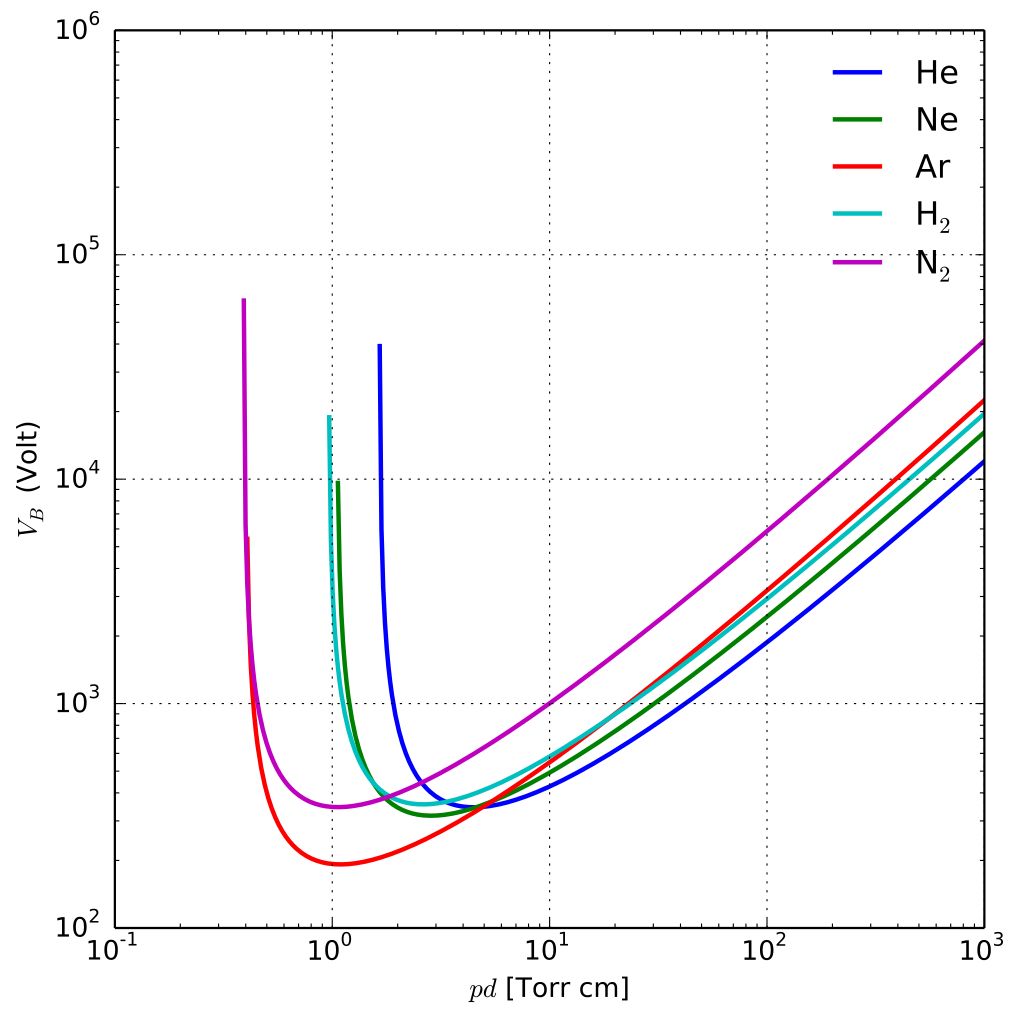
\includegraphics[scale=0.33]{./pics/pashean_lines.png}
        \caption{Эксперементальные данные Закона Пашена}
\end{figure}


%-------------------------------------------------------------------------------------------
\newpage

\section{Вывод}

\begin{equation*}
    U_{\text{пр}} = U_{\text{пр}}(lP),
\end{equation*}
\\
Разность потенциалов между электродами трубки,
при которой начинается пробой газа, есть функция произведения
давления газа на расстояние между электродами. Если в нескольких
разрядных трубках с плоскими электродами создать условия,
при которых произведения $PL$ постоянны, то для всех трубок потребуется
одна и та же разность потенциалов, чтобы вызвать газовый
разряд. Этот закон был установлен экспериментально Пашеном (1865—1947) еще до создания Таунсендом теории пробоя газа.


\end{document}
